% Provenance (never printed): enseignement scientifique premiere (2019),
% theme "La Terre, un astre singulier: la forme de la Terre" (Eratosthenes,
% meridian measurement by triangulation, the metre); see
% sources/book2/PROVENANCE.md. Every length on the ellipsoid is computed in
% figdata/grade-10/meridian_degree.py (WGS 84, ledger wgs84:ellipsoid).
\chapter{De Aarde opmeten}\label{ch:g10:measuring-the-earth}

Ga op het strand staan en kijk hoe een schip naar open zee vaart. Het wordt
niet gewoon kleiner tot je het niet meer ziet: eerst verdwijnt de romp, alsof
het schip zinkt, dan het onderste deel van de bovenbouw, en de top van de
mast gaat als laatste. De zee tussen jou en het schip is niet vlak; ze welft.
Meer dan tweeëntwintig eeuwen geleden maakte een geleerde uit Alexandrië van
een vergelijkbare waarneming --- de lengte van een schaduw op het middaguur ---
een meting van de omvang van de hele planeet. Dit hoofdstuk volgt die meting
en de metingen die erop volgden: de ketens van driehoeken die landmeters over
hele landen spanden, de expedities naar het noordpoolgebied en naar de evenaar
om uit te zoeken of de Aarde afgeplat is, de geboorte van de meter, en de
satellieten waarmee de planeet vandaag wordt opgemeten.

\begin{omfigure}
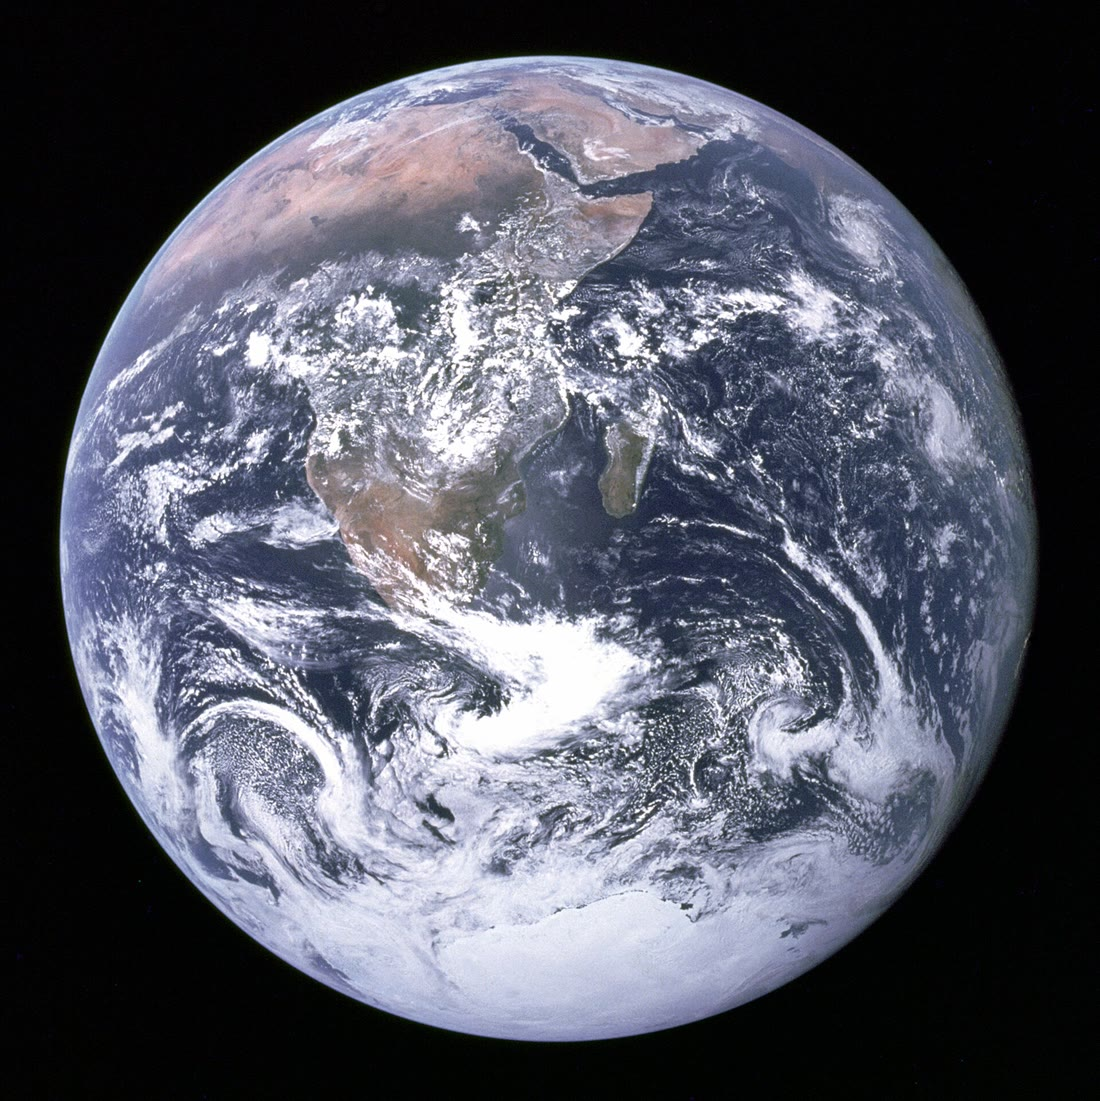
\includegraphics[width=0.5\linewidth]{images/book2/g10-nasa-apollo17-earth.jpg}

{\small De Aarde, gefotografeerd door de bemanning van Apollo~17 op weg naar de
Maan, in december 1972: Afrika, Arabië en het ijs van Antarctica. Foto:
NASA (publiek domein).}
\end{omfigure}

\begin{recall}
Een plaats op Aarde wordt vastgelegd door haar breedte, haar hoek ten noorden of
ten zuiden van de evenaar, en haar lengte, haar hoek ten oosten of ten westen van
een nulmeridiaan; meridianen verbinden de polen, breedtecirkels lopen evenwijdig
aan de evenaar rond de Aarde (Boek 1). In een homogeen medium plant licht zich
rechtlijnig voort, en de stralen die de Aarde bereiken van de zeer verre Zon
zijn evenwijdig (de natuurkundeboeken). In een rechthoekige driehoek is de
sinus van een scherpe hoek de overstaande rechthoekszijde gedeeld door de schuine
zijde, de cosinus de aanliggende rechthoekszijde gedeeld door de schuine zijde,
en de tangens de overstaande gedeeld door de aanliggende rechthoekszijde (de wiskundeboeken).
\end{recall}

\section{Een ronde Aarde}

Lang voordat iemand de Aarde vanuit de ruimte kon bekijken, lieten al
verschillende waarnemingen zien dat ze rond is.
\begin{itemize}
  \item \textbf{Schepen achter de horizon.} Een schip dat wegvaart, verdwijnt
        van onderen naar boven, in elke richting en op elke zee: het zeeoppervlak
        is overal gekromd.
  \item \textbf{De schaduw op de Maan.} Bij een maansverduistering valt de
        schaduw van de Aarde op de Maan. De rand ervan is altijd een cirkelboog,
        hoe laat het in de nacht ook is; alleen een bol werpt in elke richting
        een ronde schaduw.
  \item \textbf{De sterren veranderen met de breedte.} Wie naar het noorden
        reist, ziet de Poolster hoger boven de horizon klimmen, en sterren van
        de zuidelijke hemel verdwijnen eronder: de horizon van de reiziger
        kantelt doordat hij zich over een gekromd oppervlak verplaatst.
  \item \textbf{Reizen om de wereld en het zicht vanuit de ruimte.} Schepen, en
        later vliegtuigen, zijn in alle richtingen rond de wereld gereisd; sinds
        de jaren 1960 is de hele ronde planeet gefotografeerd.
\end{itemize}

\begin{omfigure}
\begin{tikzpicture}[font=\small, >={Stealth[length=2.2mm]}]
  % sea surface: arc of a circle of radius 8 centred at (0,-8) (curvature exaggerated)
  \fill[omDef!10] plot[domain=-4.6:4.6, samples=60] (\x,{sqrt(64-\x*\x)-8}) -- (4.6,-2.2) -- (-4.6,-2.2) -- cycle;
  \draw[omDef!70!black, thick] plot[domain=-4.6:4.6, samples=60] (\x,{sqrt(64-\x*\x)-8});
  % observer on a small tower at x=-4 (surface y=-1.072), eye at y=-0.235
  \draw[black!70, line width=1pt] (-4,-1.072) -- (-4,-0.235);
  \fill (-4,-0.235) circle (2pt);
  \node[anchor=east, align=right] at (-4.1,-0.2) {oog van de\\waarnemer};
  % line of sight tangent at x=-0.5 (y=-0.0156, slope 0.0626)
  \draw[omThm!80!black, thick] (-4,-0.235) -- (4.4,0.290);
  \node[omThm!80!black, anchor=south, rotate=3.6] at (1.3,0.1) {gezichtslijn};
  \fill[omThm!80!black] (-0.5,-0.0156) circle (1.4pt);
  % ship at x=3 (surface y=-0.584), tilted 22 degrees with the local vertical
  \begin{scope}[shift={(3,-0.584)}, rotate=-22]
    \fill[black!12] (-0.6,0) -- (0.6,0) -- (0.75,0.32) -- (-0.75,0.32) -- cycle;
    \draw[black!45, densely dashed] (-0.6,0) -- (0.6,0) -- (0.75,0.32) -- (-0.75,0.32) -- cycle;
    \draw[black!45, densely dashed] (0,0.32) -- (0,0.95);
    \draw[black!80, line width=1pt] (0,0.95) -- (0,1.55);
    \fill[black!80] (0,1.55) -- (0.32,1.25) -- (0,1.25) -- cycle;
  \end{scope}
  \node[anchor=north, align=center, font=\footnotesize] at (2.9,-1.25) {romp en onderkant mast\\verborgen achter de bolling};
  \node[anchor=north, font=\footnotesize] at (-0.5,-0.1) {horizon};
\end{tikzpicture}

{\small Waarom een schip van onderen naar boven verdwijnt: de waarnemer ziet
alleen wat boven de gezichtslijn ligt die bij de horizon langs de zee scheert.
De kromming is sterk overdreven.}
\end{omfigure}

\section{Eratosthenes meet de Aarde}

Eratosthenes van Cyrene (276--194 v.Chr.) was de bibliothecaris van
Alexandrië. Hij had gehoord dat in Syene, het huidige Aswan, ver stroomopwaarts
aan de Nijl, de Zon op de dag van de zomerzonnewende om twaalf uur 's middags
de hele bodem van een put verlichtte: ze stond dan precies in het zenit. In
Alexandrië wierp een verticale stok op hetzelfde moment een korte schaduw: de
zonnestralen maakten een hoek van ongeveer \qty{7.2}{\degree} met de verticaal,
een vijftigste van een volle cirkel.
% ledger: erat:method, erat:stadion

\begin{omfigure}
\begin{tikzpicture}[font=\small, >={Stealth[length=2.2mm]}]
  \def\R{2.4}
  \fill[omDef!8] (0,0) circle (\R);
  \draw[omDef!70!black, thick] (0,0) circle (\R);
  \coordinate (O) at (0,0);
  \coordinate (S) at (\R,0);
  \coordinate (A) at ({\R*cos(25)},{\R*sin(25)});
  \coordinate (T) at ({(\R+0.75)*cos(25)},{(\R+0.75)*sin(25)});
  \coordinate (T2) at ({(\R+1.75)*cos(25)},{(\R+1.75)*sin(25)});
  % radii
  \draw[black!70] (O) -- (S);
  \draw[black!70] (O) -- (A);
  \draw[black!40, densely dashed] (A) -- (T2);
  \fill (O) circle (1.5pt) node[below left] {middelpunt};
  % stick at Alexandria, along the radius
  \draw[line width=1.6pt, black!85] (A) -- ($(A)!0.6!(T)$);
  % well at Syene
  \draw[black!80, thick] ({\R-0.38},-0.12) -- (\R,-0.12) ($(S)+(0,0.12)$) -- ({\R-0.38},0.12);
  % parallel sun rays coming from the right
  \foreach \y in {-1.6,-0.8,0.8,1.6} \draw[->, omThm!70, thick] (6.6,\y) -- (4.4,\y);
  \draw[->, omThm!85!black, thick] (6.6,0) -- (\R+0.05,0);
  \draw[->, omThm!85!black, thick] (6.6,{(\R+0.45)*sin(25)}) -- ({(\R+0.45)*cos(25)+0.03},{(\R+0.45)*sin(25)});
  \node[omThm!85!black, align=center, anchor=west] at (4.6,2.35) {zonlicht:\\evenwijdige stralen};
  % angles
  \draw[omExo!80!black, thick] (0.75,0) arc (0:25:0.75);
  \node[omExo!80!black] at (1.05,0.22) {$\alpha$};
  \coordinate (Q) at ($(A)!0.6!(T)$);
  \draw[omExo!80!black, thick] ($(Q)+(0.8,0)$) arc (0:25:0.8);
  \node[omExo!80!black] at ($(Q)+({1.08*cos(12.5)},{1.08*sin(12.5)})$) {$\alpha$};
  \node[anchor=east] at ($(A)+(-0.12,0.18)$) {Alexandrië};
  \node[anchor=north west] at ($(S)+(0.3,-0.12)$) {Syene};
  \node[font=\footnotesize, anchor=north] at ($(O)!0.5!(S)+(0.2,-0.05)$) {};
  \draw[<->, black!60] ({(\R-0.3)*cos(3)},{(\R-0.3)*sin(3)}) arc (3:22:{\R-0.3});
  \node[anchor=east, font=\footnotesize] at ({(\R-0.35)*cos(13)},{(\R-0.35)*sin(13)}) {$d$};
\end{tikzpicture}

{\small De redenering van Eratosthenes. In Syene staat de Zon in het zenit: haar
stralen wijzen naar het middelpunt van de Aarde. In Alexandrië maakt een
verticale stok, die ook naar het middelpunt wijst, een hoek $\alpha$ met de
stralen. De hoek in het middelpunt tussen de twee plaatsen is diezelfde $\alpha$.
De hoek is overdreven: hij was maar \qty{7.2}{\degree}.}
\end{omfigure}

\begin{proposition}[De betrekking van Eratosthenes]\label{prop:g10:measuring-the-earth:eratosthenes}
Als twee plaatsen op dezelfde meridiaan liggen, op een afstand $d$ van elkaar,
en de zonnestralen op het middaguur hoeken met de verticaal maken die
$\alpha$ (in graden) verschillen, dan is de omtrek van de Aarde
\[
  C = \frac{\qty{360}{\degree}}{\alpha}\, d .
\]
\end{proposition}

\begin{proof}
De Zon staat zo ver weg dat haar stralen die de twee plaatsen bereiken
evenwijdig zijn. Op elke plaats wijst de verticaal naar het middelpunt van de
Aarde. In de figuur zijn de straal die de stok bereikt en de straal van de cirkel
door Syene twee evenwijdige lijnen, en de straal door Alexandrië snijdt ze
allebei: de hoek $\alpha$ tussen de stok en de zonnestraal en de hoek in het
middelpunt tussen de twee stralen van de cirkel zijn Z-hoeken, dus gelijk. De
boog $d$ is hetzelfde deel van de hele omtrek als de hoek $\alpha$ van een volle
cirkel: $d/C = \alpha/\qty{360}{\degree}$.
\end{proof}

\begin{method}[Een omtrek bepalen uit twee schaduwen]\label{met:g10:measuring-the-earth:shadows}
\begin{enumerate}
  \item Kies twee plaatsen op (bijna) dezelfde meridiaan en meet de
        noord-zuidafstand $d$ ertussen.
  \item Meet op dezelfde dag, om plaatselijk 12 uur 's middags, op elke plaats
        de hoek tussen een verticale stok en de zonnestralen: $\tan \theta = s/h$,
        met $h$ de hoogte van de stok en $s$ de lengte van zijn schaduw. Kijk
        nooit naar de Zon zelf: de hoek wordt alleen uit de schaduw afgelezen.
  \item Neem het verschil $\alpha$ van de twee hoeken en pas
        $C = (360/\alpha)\,d$ toe.
\end{enumerate}
\end{method}

\begin{example}[De getallen van Eratosthenes]\label{ex:g10:measuring-the-earth:numbers}
% ledger: erat:method, erat:stadion
Eratosthenes nam voor de afstand van Alexandrië naar Syene 5000
\emph{stadiën}, een Griekse lengtemaat. Met $\alpha = 1/50$ van een cirkel geldt
\[
  C = 50 \times 5000 = 250\,000 \text{ stadiën}.
\]
Hoe lang was een stadion? Historici zijn het daar nog altijd niet over eens.
Met \qty{157.2}{m} is $C \approx \qty{39300}{km}$; met \qty{166.7}{m} is
$C \approx \qty{41700}{km}$. De werkelijke meridiaanomtrek is
\qty{40008}{km}: in beide gevallen zat Eratosthenes er maar enkele procenten naast.
\end{example}

\begin{remark}[Wat werd aangenomen]\label{rem:g10:measuring-the-earth:assumptions}
Eratosthenes nam aan dat de Aarde een bol is, dat de Zon ver genoeg staat om
haar stralen evenwijdig te maken, dat Syene precies op de keerkring ligt (waar
de Zon in het zenit kan staan) en dat Syene recht ten zuiden van Alexandrië
ligt. Dat klopte telkens bijna, maar niet helemaal: Aswan ligt ongeveer
\qty{3}{\degree} lengte ten oosten van Alexandrië. Wat telt, is het
noord-zuiddeel van de afstand, het deel langs de meridiaan.
% ledger: geonames:aswan, geonames:alexandria
\end{remark}

\section{Triangulatie}

Een lange afstand op de grond meten met een meetketting of een meetlat gaat
traag, en over rivieren, bossen en bergen heen is het onmogelijk. Hoeken
daarentegen kun je heel nauwkeurig meten met een kijker op een verdeelde cirkel,
die je om beurten op twee verre seinpunten richt. Vanaf de achttiende eeuw
gebruikten landmeters dat om hele landen op te meten.

\begin{definition}[Geodesie]\label{def:g10:measuring-the-earth:geodesy}
\emph{Geodesie}\index{geodesie} is de wetenschap die de vorm en de afmetingen
van de Aarde en de ligging van punten op haar oppervlak meet, en volgt hoe die
in de loop van de tijd veranderen.
\end{definition}

\begin{definition}[Triangulatie]\label{def:g10:measuring-the-earth:triangulation}
\emph{Triangulatie}\index{triangulatie} bepaalt de ligging van verre punten met
een keten van driehoeken: één zijde, de \emph{basislijn}, wordt heel zorgvuldig
op de grond gemeten; alle hoeken van de driehoeken worden vanuit hun hoekpunten
gemeten; elke andere zijde wordt daarna berekend.
\end{definition}

De berekening steunt op één betrekking tussen de zijden en de hoeken van een
willekeurige driehoek. In een driehoek $ABC$ noemen we $a$, $b$, $c$ de zijden
tegenover de hoekpunten $A$, $B$, $C$, en ook de hoeken bij die hoekpunten
noemen we $A$, $B$, $C$.

\begin{proposition}[De sinusregel]\label{prop:g10:measuring-the-earth:sine-rule}
In elke driehoek $ABC$ geldt
\[
  \frac{a}{\sin A} = \frac{b}{\sin B} = \frac{c}{\sin C}.
\]
\end{proposition}

\begin{proof}
Trek de hoogtelijn uit $C$, die de lijn $AB$ snijdt in $H$ (tweede deel van de
figuur hieronder); noem $h = CH$. In de rechthoekige driehoek $AHC$ is
$\sin A = h/b$, dus $h = b \sin A$. In de rechthoekige driehoek $BHC$ is
$\sin B = h/a$, dus $h = a \sin B$. Dus $b \sin A = a \sin B$, dat wil zeggen
$a/\sin A = b/\sin B$. (Is de hoek bij $B$ stomp, dan valt $H$ voorbij $B$ en is
de hoek van de rechthoekige driehoek bij $B$ gelijk aan $\qty{180}{\degree} - B$,
die dezelfde sinus heeft.) Hetzelfde argument met de hoogtelijn uit $A$ geeft
$b/\sin B = c/\sin C$.
\end{proof}

\begin{omfigure}
\begin{tikzpicture}[font=\small, >={Stealth[length=2mm]}]
  \begin{scope}
    \coordinate (A) at (0,0); \coordinate (B) at (2.0,0.25);
    \coordinate (C) at (0.9,1.9); \coordinate (D) at (3.0,2.1);
    \coordinate (E) at (1.9,3.8); \coordinate (F) at (3.9,4.1);
    \coordinate (G) at (2.7,5.6);
    \draw[black!60] (A) -- (C) -- (B) (C) -- (D) -- (B) (C) -- (E) -- (D) -- (F) -- (E) -- (G) -- (F);
    \draw[omThm!85!black, line width=2pt] (A) -- (B);
    \foreach \p in {A,B,C,D,E,F,G} \fill (\p) circle (1.6pt);
    \node[below left] at (A) {$A$}; \node[below right] at (B) {$B$};
    \node[left] at (C) {$C$}; \node[right] at (D) {$D$};
    \node[left] at (E) {$E$}; \node[right] at (F) {$F$}; \node[above] at (G) {$G$};
    \node[omThm!85!black, anchor=north, font=\footnotesize] at (1.25,-0.3) {gemeten basislijn};
    \draw[omExo!80!black] ($(A)!0.28!(B)$) arc[start angle=7, end angle=64.6, radius=0.56];
    \draw[omExo!80!black] ($(B)!0.3!(A)$) arc[start angle=187, end angle=123, radius=0.6];
    \draw[black!50, densely dashed] (-0.5,0) -- (-0.5,5.6);
    \draw[->, black!70] (-0.5,5.0) -- (-0.5,5.8) node[above] {N};
    \node[rotate=90, font=\footnotesize, black!60, anchor=south] at (-0.5,2.6) {meridiaan};
  \end{scope}
  \begin{scope}[xshift=6.2cm, yshift=0.6cm]
    \coordinate (A) at (0,0); \coordinate (B) at (4,0); \coordinate (C) at (1.4,2.6);
    \coordinate (H) at (1.4,0);
    \draw[thick] (A) -- (B) -- (C) -- cycle;
    \draw[omDef!80!black, densely dashed] (C) -- (H);
    \draw[omDef!80!black] (1.4,0.22) -- (1.62,0.22) -- (1.62,0);
    \node[below left] at (A) {$A$}; \node[below right] at (B) {$B$};
    \node[above] at (C) {$C$}; \node[below] at (H) {$H$};
    \node[omDef!80!black, anchor=west] at (1.4,1.05) {$h$};
    \node[anchor=south east] at (0.7,1.3) {$b$};
    \node[anchor=south west] at (2.75,1.35) {$a$};
    \node[anchor=north] at (2.7,-0.02) {$c$};
    \draw[omExo!80!black] (0.5,0) arc (0:61.7:0.5);
    \draw[omExo!80!black] (3.45,0) arc (180:135:0.55);
  \end{scope}
\end{tikzpicture}

{\small Links: een keten van driehoeken langs een meridiaan, vanaf een gemeten
basislijn $AB$; de boogjes geven twee van de vele hoeken aan die met het
instrument zijn gemeten. Rechts: de hoogte $h$ uit $C$, op twee manieren
uitgedrukt, levert de sinusregel.}
\end{omfigure}

\begin{method}[Een triangulatieketen doorrekenen]\label{met:g10:measuring-the-earth:chain}
\begin{enumerate}
  \item In de eerste driehoek $ABC$ worden de basislijn $c = AB$ en de hoeken
        bij $A$ en $B$ gemeten; de derde hoek is
        $C = \qty{180}{\degree} - A - B$ (en zijn meting controleert de
        andere).
  \item De sinusregel geeft de twee andere zijden:
        $b = AC = c \sin B / \sin C$ en $a = BC = c \sin A / \sin C$.
  \item Een berekende zijde wordt de bekende zijde van de volgende driehoek,
        en zo verder langs de keten.
  \item Ten slotte wordt het noord-zuiddeel van elke zijde berekend met de
        cosinus van haar hoek met de meridiaan, en worden de delen opgeteld.
\end{enumerate}
\end{method}

\begin{example}[Eén driehoek]\label{ex:g10:measuring-the-earth:triangle}
Er wordt een basislijn $AB = \qty{8.000}{km}$ gemeten; vanuit $A$ wordt het
seinpunt $C$ gezien onder \qty{70}{\degree} met de richting van $B$, vanuit $B$
onder \qty{60}{\degree} met de richting van $A$. Dan is $C = \qty{50}{\degree}$ en
\[
  AC = \frac{8.000 \times \sin 60^\circ}{\sin 50^\circ} = \frac{8.000 \times 0.8660}{0.7660}
  \approx \qty{9.044}{km}, \qquad
  BC = \frac{8.000 \times \sin 70^\circ}{\sin 50^\circ} \approx \qty{9.814}{km}.
\]
Behalve de basislijn is er geen enkele afstand te voet afgelegd.
\end{example}

\begin{example}[De meridiaan van de meter]\label{ex:g10:measuring-the-earth:meridian}
% ledger: metre:1791, metre:survey, geonames:dunkirk, geonames:barcelona (arc computed in figdata/grade-10/meridian_degree.py)
In maart 1791 werd de meter gedefinieerd als een tienmiljoenste van de afstand
van de pool tot de evenaar langs een meridiaan. Om die afstand te vinden, maten
twee astronomen, Jean-Baptiste Delambre en Pierre Méchain, met \omterm{def:g10:measuring-the-earth:triangulation}{triangulatie} de
meridiaanboog van Duinkerke, aan de Noordzee, tot Barcelona, aan de
Middellandse Zee --- bijna zeven jaar werk, Delambre in de noordelijke twee
derde, Méchain in het zuidelijke derde. De twee steden verschillen
\qty{9.646}{\degree} in breedte; op de moderne ellipsoïde is de boog tussen
hun breedtecirkels \qty{1072.2}{km} lang. Uit de lengte van een boog en zijn
breedteverschil volgt de lengte van een graad; de vorm van de Aarde geeft dan
de hele kwartmeridiaan. In 1799 werden platina standaarden van de nieuwe meter
gemaakt en in de nationale archieven bewaard.
\end{example}

\begin{history}[De herhalingscirkel]
De hoeken van de meridiaan van de meter werden gemeten met een
\emph{herhalingscirkel}, een instrument van Jean-Charles de Borda: twee
kijkers op een verdeelde cirkel, die vele malen beurtelings op twee seinpunten
worden gericht, zodat de afleesfouten van de schaalverdeling worden gedeeld
door het aantal herhalingen.
\begin{center}
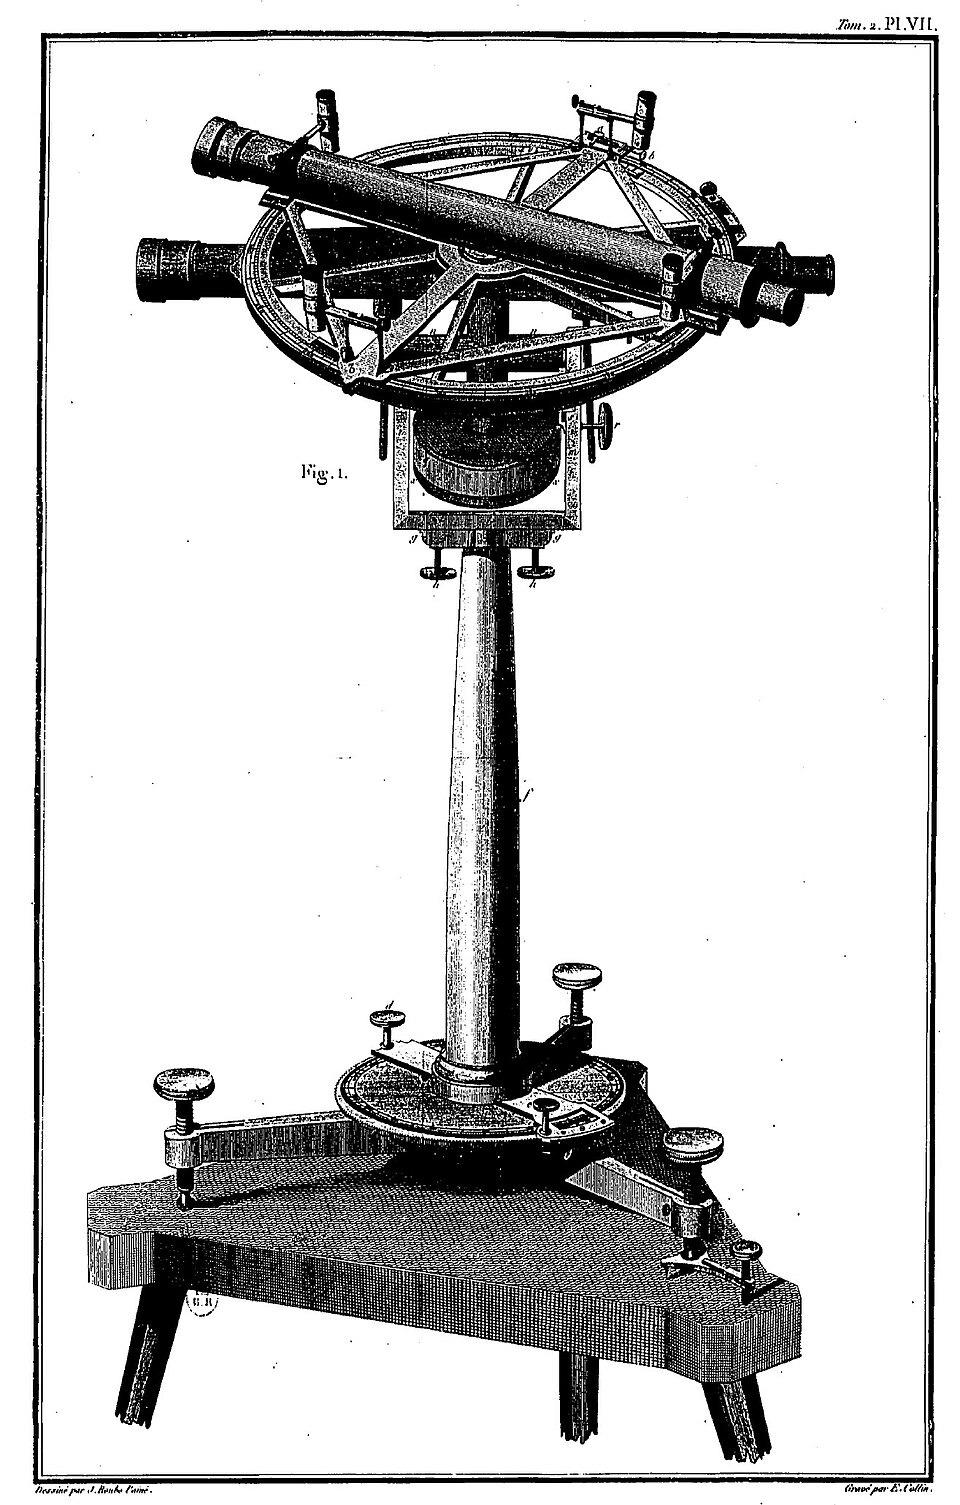
\includegraphics[width=0.3\linewidth]{images/book2/g10-delambre-repeating-circle.jpg}

{\small Een herhalingscirkel, opgesteld om horizontale hoeken te meten, zoals
gegraveerd in Delambres verslag van de meting (1807). Publiek domein (Wikimedia
Commons).}
\end{center}
\end{history}

\section{Een afgeplatte Aarde}

Rond 1687 betoogde Isaac Newton op grond van zijn gravitatietheorie dat een
draaiende Aarde een bij de polen afgeplatte en bij de evenaar uitpuilende
sferoïde moet zijn. Gradenmetingen langs de meridiaan door de astronomen van
de sterrenwacht van Parijs leken het tegendeel te zeggen: een Aarde die bij de
polen uitgerekt is. De vraag werd beslist door de lengte van één breedtegraad
zo ver mogelijk uit elkaar te meten.
% ledger: figure:expeditions

\begin{omfigure}
\begin{tikzpicture}[font=\small, >={Stealth[length=2mm]}]
  \def\a{3.0} \def\b{2.3}
  \draw[black!35, densely dashed] (0,0) circle (\a);
  \fill[omDef!8] (0,0) ellipse ({\a} and {\b});
  \draw[omDef!70!black, thick] (0,0) ellipse ({\a} and {\b});
  \draw[black!50] (-3.4,0) -- (3.7,0);
  \draw[black!50] (0,-2.6) -- (0,3.3);
  \draw[<->, omThm!85!black] (0,-0.3) -- (\a,-0.3);
  \node[omThm!85!black, below] at (1.5,-0.3) {$a$};
  \draw[<->, omThm!85!black] (-0.3,0) -- (-0.3,\b);
  \node[omThm!85!black, left] at (-0.3,1.15) {$b$};
  \node[above right] at (0,\b) {N};
  \node[anchor=south east] at (3.0,-2.5) {};
  \node[anchor=west] at (3.7,0) {evenaar};
  % normal at t = 45 deg: P = (2.121, 1.626); crosses the equator at (0.874,0), the axis at (0,-1.14)
  \coordinate (P) at (2.121,1.626);
  \draw[omExo!85!black, thick] (P) -- ($(P)!1.35!(0.874,0)$);
  \draw[omExo!85!black, thick, ->] (P) -- ($(P)!-0.45!(0.874,0)$);
  \fill (P) circle (1.6pt);
  \node[anchor=west, align=left, font=\footnotesize] at (2.85,2.35) {plaatselijke verticaal\\(schietlood)};
  \draw[omExo!85!black] (1.45,0) arc (0:52.5:0.58);
  \node[omExo!85!black] at (1.62,0.32) {$\varphi$};
  \fill (0,0) circle (1.3pt);
  \node[anchor=north east, font=\footnotesize] at (0,0) {middelpunt};
  \node[black!50, font=\footnotesize, anchor=south] at (-2.2,2.15) {bol};
\end{tikzpicture}

{\small Een afgeplatte Aarde, met de \omterm{def:g10:measuring-the-earth:ellipsoid}{afplatting} sterk overdreven (de werkelijke
is op deze schaal te klein om te zien). De verticaal op een plaats staat
loodrecht op het oppervlak; ze wijst niet precies naar het middelpunt. De
breedte $\varphi$ van de plaats is de hoek tussen haar verticaal en het vlak
van de evenaar.}
\end{omfigure}

De breedte wordt aan de sterren gemeten: het is de hoek tussen de plaatselijke
verticaal en het vlak van de evenaar. Op een afgeplatte Aarde is het oppervlak
bij de polen minder gekromd dan bij de evenaar. Waar het oppervlak minder
gekromd is, moet je er verder over reizen voordat de verticaal één graad
draait: \emph{een breedtegraad is bij de polen langer}.

\begin{history}[Lapland en Peru]
% ledger: figure:expeditions, figure:degrees
In 1735 stuurde de Academie van Wetenschappen van Parijs een expeditie naar de
evenaar, naar de Spaanse provincie Peru (nu Ecuador); ze werkte daar negen jaar,
tot 1744. In 1736--1737 mat een tweede expeditie, onder leiding van
Pierre-Louis Moreau de Maupertuis en met de jonge wiskundige Alexis Clairaut,
een meridiaangraad in Lapland, bij de noordpoolcirkel. De graad in Lapland
kwam uit op 57\,437 \emph{toises} (de oude lengtemaat; ongeveer
\qty{111.95}{km}), de graad in Peru op maar 56\,737 toises: bij de pool is de
graad langer, en Newton had gelijk. De twee getallen wezen op een \omterm{def:g10:measuring-the-earth:ellipsoid}{afplatting}
van ongeveer $1/205$ --- te groot, zoals latere metingen lieten zien, maar de
vraag naar het teken was beslist.
\end{history}

\begin{omfigure}
\begin{tikzpicture}
\begin{axis}[omrecord, width=0.82\linewidth, height=5.4cm, xmin=0, xmax=90,
  ymin=110.45, ymax=111.8, xlabel={breedte (\unit{\degree})},
  ylabel={lengte van \qty{1}{\degree} breedte (km)}, xtick={0,15,...,90},
  ytick={110.6,110.8,...,111.8}, yticklabel style={/pgf/number format/fixed, /pgf/number format/fixed zerofill, /pgf/number format/precision=1}]
\addplot[omDef!85!black, line width=1.1pt] table[x=lat_deg, y=deg_km] {figdata/out/grade-10-meridian_degree.dat};
\addplot[only marks, mark=*, mark size=1.8pt, omThm!85!black] coordinates {(0,110.574) (45,111.132) (66,111.507) (90,111.694)};
\node[anchor=south west, font=\footnotesize] at (axis cs:2,110.6) {110.57 km};
\node[anchor=north east, font=\footnotesize] at (axis cs:89,111.56) {111.69 km};
\node[anchor=north west, font=\footnotesize] at (axis cs:46,111.12) {111.13 km};
\node[anchor=south east, font=\footnotesize] at (axis cs:65,111.53) {111.51 km op \ang{66} (Lapland)};
\end{axis}
\end{tikzpicture}

{\small De lengte van één breedtegraad op de \omterm{def:g10:measuring-the-earth:ellipsoid}{referentie-ellipsoïde} van
\cref{def:g10:measuring-the-earth:ellipsoid}, van de evenaar tot de pool.
Berekend met de WGS~84-ellipsoïde.}
\end{omfigure}

\begin{definition}[Referentie-ellipsoïde en afplatting]\label{def:g10:measuring-the-earth:ellipsoid}
Een \emph{referentie-ellipsoïde}\index{referentie-ellipsoide@referentie-ellipsoïde} is het oppervlak
dat ontstaat door een ellips om haar korte as te laten draaien, zo gekozen dat
het zo goed mogelijk bij de vorm van de Aarde past. Haar \emph{equatoriale straal}
is $a$, haar \emph{poolstraal} $b$, en haar
\emph{afplatting}\index{afplatting} is
\[
  f = \frac{a-b}{a}.
\]
\end{definition}

\begin{proposition}[De afmetingen van de Aarde]\label{prop:g10:measuring-the-earth:dimensions}
% ledger: wgs84:ellipsoid, earth:Req, earth:Rpol, earth:Rmean (lengths computed in figdata/grade-10/meridian_degree.py)
De \omterm{def:g10:measuring-the-earth:ellipsoid}{referentie-ellipsoïde} die satellietplaatsbepaling gebruikt (WGS~84), heeft
\[
  a = \qty{6378.137}{km}, \qquad b = \qty{6356.752}{km}, \qquad
  f = \frac{1}{298.257}.
\]
De poolstraal is \qty{21.4}{km} korter dan de equatoriale straal. De evenaar
is \qty{40075}{km} lang en een meridiaan, van pool tot pool en terug,
\qty{40008}{km}; de kwartmeridiaan, van de evenaar tot een pool, is
\qty{10001.966}{km}. Eén breedtegraad is \qty{110.574}{km} lang bij de
evenaar en \qty{111.694}{km} bij de polen. Een lengtegraad is op de evenaar
\qty{111.32}{km} lang en krimpt naar de polen toe ongeveer als
$\cos \varphi$.
\end{proposition}

\begin{example}[Een lengtegraad]\label{ex:g10:measuring-the-earth:longitude}
Een breedtecirkel op breedte $\varphi$ is een cirkel met als straal de afstand
tot de as, ongeveer $R \cos \varphi$. Op \qty{60}{\degree} NB is zijn omtrek
ongeveer de helft van die van de evenaar, en een lengtegraad is ongeveer
$111.32 \times \cos 60^\circ \approx \qty{55.7}{km}$ (de ellipsoïde geeft
\qty{55.80}{km}).
\end{example}

\begin{remark}[Hoe rond is rond?]\label{rem:g10:measuring-the-earth:round}
Een \omterm{def:g10:measuring-the-earth:ellipsoid}{afplatting} van $1/298$ is klein. Op een globe met een doorsnede van
\qty{30}{cm} zou de pooldiameter maar \qty{1}{mm} korter zijn dan de
equatoriale --- onzichtbaar. De diepste oceaantrog, bijna \qty{11}{km} onder
zeeniveau, zou een kras van ongeveer een kwart millimeter diep zijn. Voor de
meeste doeleinden is de Aarde een bol met een gemiddelde straal van
\qty{6371}{km}; voor nauwkeurige posities is de ellipsoïde nodig.
% ledger: earth:Rmean, usgs:trench-depth
\end{remark}

\section{Geodesie vandaag}

\begin{omfigure}
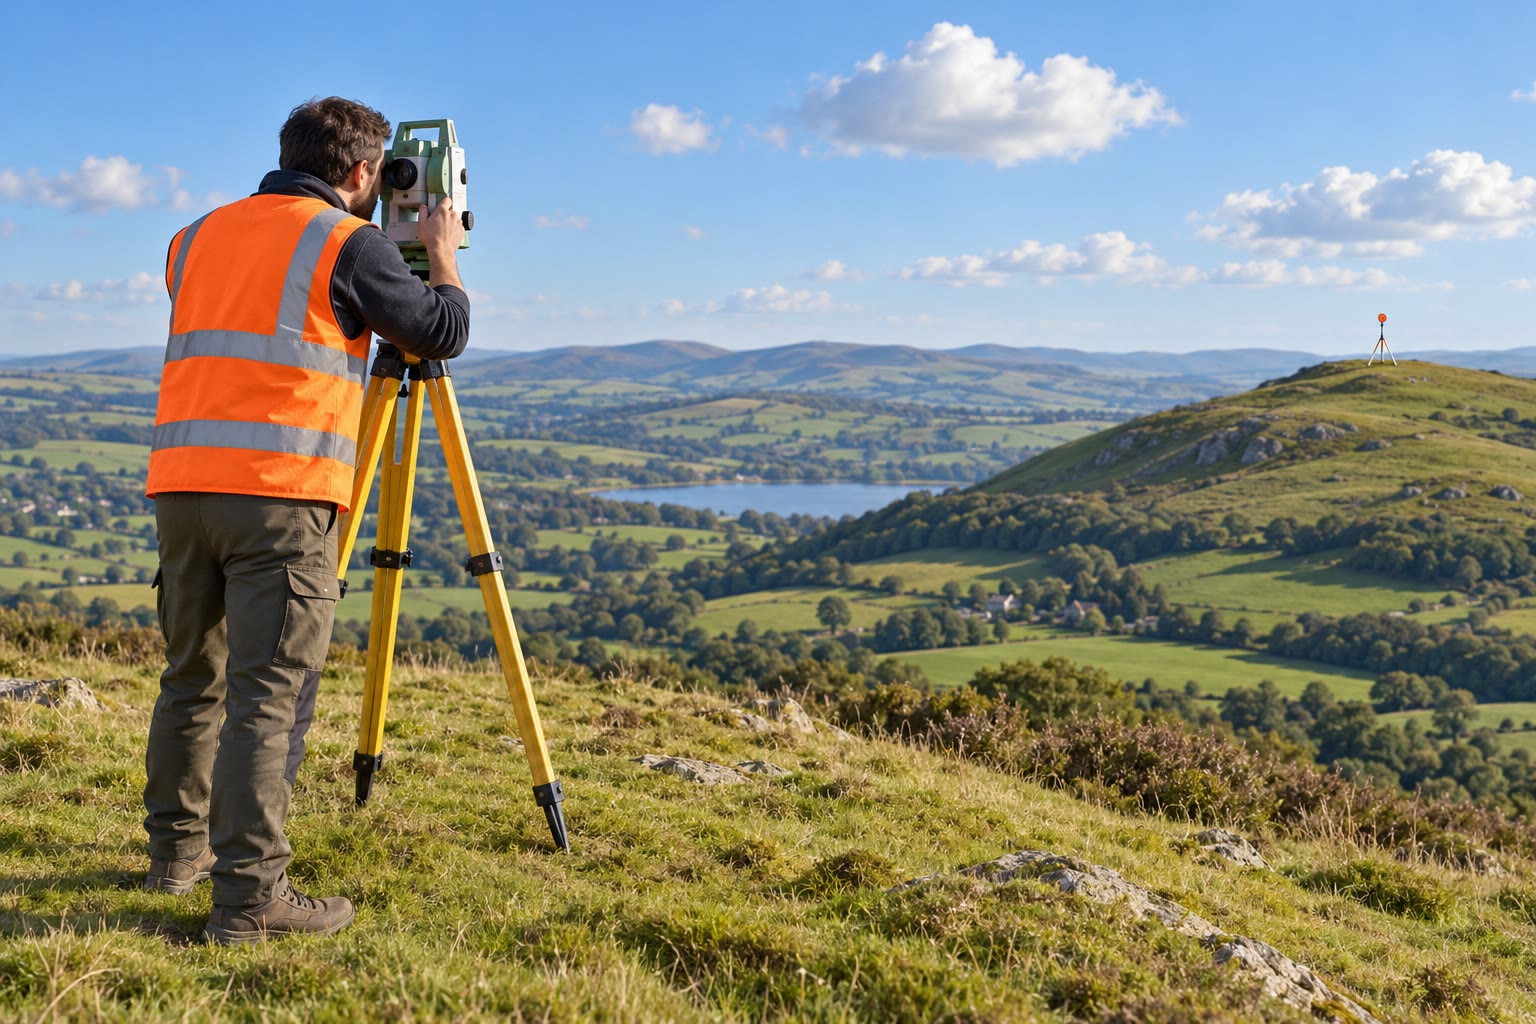
\includegraphics[width=0.7\linewidth]{images/book2/ai/g10-surveyor-theodolite.jpg}

{\small Een landmeter aan het werk met een modern instrument dat hoeken meet
en, met een lichtbundel, afstanden; op de heuvel in de verte staat een
meetsein.}
\end{omfigure}

De grote \omterm{def:g10:measuring-the-earth:triangulation}{triangulaties} van de achttiende en negentiende eeuw zijn vervangen
door satellieten. Een ontvanger op de grond vangt de signalen op van
verschillende satellieten waarvan de posities op elk ogenblik bekend zijn, en
berekent zijn eigen positie uit de looptijden van de signalen (Boek 1).
Netwerken van vaste ontvangers, over de hele wereld in het vaste gesteente
verankerd, meten hun posities voortdurend. Ze bepalen het referentiestelsel
waarin elke kaart en elke satellietpositie wordt gegeven, en ze bewegen: ze
laten zien dat de platen van de lithosfeer enkele centimeters per jaar
verschuiven (\cref{ch:g11:plate-motions}).
% ledger: usgs:gps

\begin{inthefield}[De grond vandaag opmeten]
Geodeten verankeren antennes op betonnen pijlers in het vaste gesteente, ver
van gebouwen en bomen, en registreren jarenlang om de paar seconden hun
positie. Ze combineren dat met metingen van radiotelescopen die zeer verre
sterrenstelsels waarnemen, en met laserbundels die op satellieten met
spiegels worden afgevuurd. Landmeters op bouwplaatsen en op het platteland
meten nog altijd hoeken en afstanden met instrumenten op statieven, en sluiten
die aan op het satellietstelsel.
\end{inthefield}

\section{Oefeningen}

\begin{exercise}[$\star$]\label{exo:g10:measuring-the-earth:1}
Geef drie waarnemingen, mogelijk zonder van de grond te gaan, die laten zien
dat de Aarde rond is. Leg voor elke waarneming in één zin uit waarom een platte
Aarde haar niet zou kunnen opleveren.
\end{exercise}

\begin{exercise}[$\star$]\label{exo:g10:measuring-the-earth:2}
Wat is \omterm{def:g10:measuring-the-earth:geodesy}{geodesie}? Wat is \omterm{def:g10:measuring-the-earth:triangulation}{triangulatie}, en welke ene lengte moet bij een
\omterm{def:g10:measuring-the-earth:triangulation}{triangulatie} op de grond worden gemeten?
\end{exercise}

\begin{exercise}[$\star$]\label{exo:g10:measuring-the-earth:3}
Eratosthenes vond dat de hoek tussen de zonnestralen en de verticaal in
Alexandrië $1/50$ van een volle cirkel was, terwijl de Zon in het zenit stond in
Syene, 5000 stadiën verderop. Bereken de omtrek in stadiën en daarna in
kilometer, met een stadion van \qty{157.2}{m}.
\end{exercise}

\begin{exercise}[$\star$]\label{exo:g10:measuring-the-earth:4}
Eén breedtegraad is ongeveer \qty{111}{km} lang. Hoe lang is één boogminuut
breedte ($1/60$ van een graad)? Hoe lang is de meridiaan van de evenaar tot de
pool, ongeveer?
\end{exercise}

\begin{exercise}[$\star$]\label{exo:g10:measuring-the-earth:5}
Bereken met de equatoriale straal \qty{6378.137}{km} en de poolstraal
\qty{6356.752}{km} het verschil tussen de twee stralen en de \omterm{def:g10:measuring-the-earth:ellipsoid}{afplatting}
$f = (a-b)/a$. Schrijf $f$ als één gedeeld door een geheel getal.
\end{exercise}

\begin{exercise}[$\star\star$]\label{exo:g10:measuring-the-earth:6}
Twee steden liggen op dezelfde meridiaan, \qty{500}{km} uit elkaar. Om
12 uur 's middags op dezelfde dag werpt een verticale stok van \qty{1.00}{m}
hoog een schaduw van \qty{0.364}{m} in de zuidelijke stad en van
\qty{0.456}{m} in de noordelijke stad. Bereken in elke stad de hoek tussen de
zonnestralen en de verticaal, en daarna de omtrek van de Aarde.
\end{exercise}

\begin{exercise}[$\star\star$]\label{exo:g10:measuring-the-earth:7}
In een driehoek $ABC$ is de basislijn $AB = \qty{10.00}{km}$, de hoek bij $A$
\qty{62}{\degree} en de hoek bij $B$ \qty{71}{\degree}. Bereken de hoek bij $C$
en de lengtes $AC$ en $BC$.
\end{exercise}

\begin{exercise}[$\star\star$]\label{exo:g10:measuring-the-earth:8}
Een vliegtuig vliegt recht naar het westen langs de breedtecirkel
\qty{60}{\degree} NB, van \qty{10}{\degree} OL naar \qty{20}{\degree} WL.
Bereken met een lengtegraad van $111.3 \cos \varphi$ km de afstand die het
aflegt. Hoe lang zou dezelfde verandering in lengte op de evenaar zijn?
\end{exercise}

\begin{exercise}[$\star\star$]\label{exo:g10:measuring-the-earth:9}
Het oog van een waarnemer bevindt zich $h = \qty{2}{m}$ boven een kalme zee. De
gezichtslijn naar de horizon scheert in $T$ langs de zee; het middelpunt van de
Aarde is $O$, het oog $E$. Leg uit waarom de driehoek $OTE$ in $T$ een rechte
hoek heeft, en laat dan met de stelling van Pythagoras en $R = \qty{6371}{km}$
zien dat de afstand tot de horizon ongeveer $\sqrt{2Rh}$ is. Bereken die.
\end{exercise}

\begin{exercise}[$\star\star$]\label{exo:g10:measuring-the-earth:10}
Lees de kromme van de graadlengtes af. Tussen welke breedtes verandert de
lengte van een graad het snelst? Leg in twee zinnen uit waarom een breedtegraad
bij de polen langer is dan bij de evenaar.
\end{exercise}

\begin{exercise}[$\star\star$]\label{exo:g10:measuring-the-earth:11}
De meridiaanboog van Duinkerke tot Barcelona overspant \qty{9.646}{\degree}
breedte en is \qty{1072.2}{km} lang. Bereken de gemiddelde lengte van een graad
langs deze boog. Hoe lang zou de kwartmeridiaan zijn als elke graad die lengte
had? Vergelijk met \qty{10002.0}{km} en verklaar het kleine verschil.
\end{exercise}

\begin{exercise}[$\star\star\star$]\label{exo:g10:measuring-the-earth:12}
Eratosthenes mat een hoek van \qty{7.2}{\degree} en een afstand van 5000
stadiën. Als zijn hoek \qty{0.1}{\degree} fout was geweest (te klein), hoeveel
procent zou zijn omtrek dan fout zijn geweest, en in welke richting? Welke van
zijn twee metingen was volgens jou de minst nauwkeurige?
\end{exercise}

\begin{exercise}[$\star\star\star$]\label{exo:g10:measuring-the-earth:13}
Een keten van twee driehoeken: in $ABC$ is $AB = \qty{6.000}{km}$,
$A = \qty{55}{\degree}$, $B = \qty{75}{\degree}$. In de volgende driehoek $ACD$,
gebouwd op de zijde $AC$, is de hoek bij $A$ \qty{50}{\degree} en de hoek bij
$C$ \qty{68}{\degree}. Bereken $AC$ en daarna $AD$.
\end{exercise}

\begin{exercise}[$\star\star\star$]\label{exo:g10:measuring-the-earth:14}
Op welke breedte is een lengtegraad half zo lang als op de evenaar? Op welke
breedte is hij een tiende zo lang? Leg uit waarom geen van beide antwoorden
afhangt van de grootte van de Aarde.
\end{exercise}

\begin{exercise}[$\star\star\star$]\label{exo:g10:measuring-the-earth:15}
Gebruik de waarden van de ellipsoïde: een breedtegraad is \qty{110.574}{km}
bij de evenaar en \qty{111.694}{km} bij de pool. Op een bol met dezelfde
gemiddelde straal zou een graad overal \qty{111.195}{km} zijn. Hoeveel meter
zou een landmeter die een bol aannam, zich vergissen over één graad bij de
evenaar, en over één graad bij de pool? Waarom moet een kaart die posities tot
op de meter geeft, op de ellipsoïde worden berekend?
\end{exercise}

\section{Probleem: de meter en de meridiaan}

\begin{problem}[{Weekendprobleem --- van de schaduw van Eratosthenes tot de
lengte van de eerste meter}]
\label{pb:g10:measuring-the-earth:1}
% ledger: geonames:aswan, geonames:alexandria, erat:method, metre:1791, metre:survey, wgs84:ellipsoid (arc lengths and degree lengths computed in figdata/grade-10/meridian_degree.py)
Een leerling volgt de geschiedenis van het opmeten van de Aarde opnieuw, met
moderne getallen. Aswan, het oude Syene, ligt op \qty{24.09}{\degree} NB en
Alexandrië op \qty{31.20}{\degree} NB; op de moderne ellipsoïde is de
meridiaanboog tussen hun twee breedtecirkels \qty{788}{km} lang. Op de
ellipsoïde meet één breedtegraad \qty{110.57}{km} bij de evenaar,
\qty{111.13}{km} op \qty{45}{\degree} en \qty{111.51}{km} op
\qty{66}{\degree}, en de kwartmeridiaan is
\qty{10001.966}{km}.

\medskip
\noindent\textbf{Deel I --- Opnieuw Eratosthenes.}
\begin{enumerate}
  \item Bereken het breedteverschil tussen Aswan en Alexandrië.
  \item Welk deel van een volle cirkel is dat? Vergelijk met de $1/50$ van
        Eratosthenes.
  \item Bereken de omtrek van de Aarde die de methode van Eratosthenes met
        deze moderne getallen oplevert.
  \item De twee steden liggen niet op dezelfde meridiaan: Aswan ligt ongeveer
        \qty{3}{\degree} lengte ten oosten van Alexandrië. Welke afstand moet
        in de methode worden gebruikt: de rechte afstand tussen de steden of
        de meridiaanboog tussen hun breedtecirkels? Waarom?
  \item Waarom moeten de twee schaduwen op dezelfde dag, om plaatselijk
        12 uur 's middags, worden gemeten?
\end{enumerate}

\medskip
\noindent\textbf{Deel II --- Een kleine triangulatie.}
Er wordt een basislijn $AB = \qty{12.000}{km}$ gemeten. Vanuit $A$ wordt het
seinpunt $C$ gezien onder \qty{58}{\degree} met $B$; vanuit $B$ onder
\qty{66}{\degree} met $A$. In de volgende driehoek $ACD$ is de hoek bij $A$
\qty{47}{\degree} en de hoek bij $C$ \qty{75}{\degree}. De zijde $AD$ wijst
\qty{8}{\degree} ten oosten van het noorden.
\begin{enumerate}[resume]
  \item Bereken de hoek bij $C$ in de driehoek $ABC$.
  \item Bereken de zijde $AC$.
  \item Bereken de zijde $BC$.
  \item Bereken de hoek bij $D$ in de driehoek $ACD$, en daarna de zijde $AD$.
  \item Bereken de noord-zuidafstand tussen $A$ en $D$.
  \item Bereken met de graadlengte op \qty{45}{\degree} het breedteverschil
        tussen $A$ en $D$, in graden en in boogminuten.
\end{enumerate}

\medskip
\noindent\textbf{Deel III --- Een afgeplatte Aarde.}
\begin{enumerate}[resume]
  \item Hoeveel meter is een breedtegraad op \qty{66}{\degree} langer dan een
        breedtegraad bij de evenaar?
  \item Leg uit wat dit verschil zegt over de vorm van de Aarde.
  \item Op de ellipsoïde is $a = \qty{6378.137}{km}$ en
        $b = \qty{6356.752}{km}$. Bereken $a - b$ en de \omterm{def:g10:measuring-the-earth:ellipsoid}{afplatting}.
  \item Leg uit waarom het schietlood op een afgeplatte Aarde, op een plaats op
        \qty{45}{\degree} breedte, niet precies naar het middelpunt van de
        Aarde wijst.
\end{enumerate}

\medskip
\noindent\textbf{Deel IV --- De eerste meter.}
\begin{enumerate}[resume]
  \item Hoe lang zou de kwartmeridiaan volgens de definitie van 1791 moeten
        zijn, in meter?
  \item De platina meter van 1799 werd gemaakt op basis van een gemeten waarde
        van de meridiaan. Als de kwartmeridiaan in werkelijkheid
        \qty{10001.966}{km} is, hoe lang is dan een tienmiljoenste ervan?
  \item Was de meter van 1799 te lang of te kort vergeleken met zijn eigen
        definitie? Met welk deel?
  \item De platina staaf gaf getrouw de lengte weer die in de jaren 1790 was
        berekend. Was de kwartmeridiaan die toen werd berekend, te lang of te
        kort? Leg uit.
  \item Hoeveel millimeter was de eerste meter korter dan een tienmiljoenste
        van de werkelijke kwartmeridiaan? Vergelijk met de dikte van een vel
        papier, ongeveer \qty{0.1}{mm}.
\end{enumerate}
\end{problem}
